\documentclass{article}
\usepackage{graphicx}
\usepackage{float}
\usepackage[utf8]{inputenc}
\usepackage[spanish]{babel}
\usepackage[separate-uncertainty=true]{siunitx}
\usepackage{derivative}
%\usepackage{geometry}
\usepackage{nameref}
\usepackage[bookmarks = true, colorlinks=true, linkcolor = black, citecolor =
black, menucolor = black, urlcolor = black]{hyperref} 
\usepackage{csquotes}
\usepackage{multicol}
\setlength{\parskip}{6mm}
\usepackage{geometry}
\usepackage{biblatex}

\geometry{
   left = 15mm,
   right = 15mm,
   top = 10mm,
   bottom = 20mm
}

\addbibresource{bibliografia.bib}

\title{Caracterización de un resonador piezoeléctrico.}
\author{
    Javier Garcia Cueto \\
    \href{mailto:javigarcia2909@gmail.com}{javigarcia2909@gmail.com} 
    \and 
    Jorge Theodorou \\
    \href{mailto:jorgetheodorou@gmail.com}{jorgetheodorou@gmail.com}
    \and 
    Marcos Ruben Sidoruk \\
    \href{mailto:marcsid2003@gmail.com}{marcsid2003@gmail.com} 
}

\begin{document}

\maketitle

\begin{abstract}
A lo largo de este informe se estudia el comportamiento de un resonador
    piezoeléctrico. Se lo caracteriza como un circuito RLC serie con una
    capacitancia en paralelo al mismo, encontrando sus frecuencias de
    resonancia y antirresonancia en $\omega_R=(50082\pm1)\,$Hz y en
    $\omega_A=(50280\pm)\,$Hz al alimentarlo con una fuente de corriente
    alterna. Se observa que, de acuerdo a lo esperado, la impedancia
    equivalente del circuito se minimiza cuando la frecuencia es igual a
    $\omega_R$, y se maximiza cuando es igual a $\omega_A$. Para finalizar, se
    observa que el modelo anteriormente mencionado se ajusta correctamente a la
    señal medida a la salida del circuito.
\end{abstract}

\section{Introducción} 

\paragraph{} 
Un material piezoeléctrico se caracteriza por producir una
polarización eléctrica (y por lo tanto, un campo eléctrico) al ser sometido a
compresiones mecánicas \cite{guia_piezoelectrico}. De modo inverso, si se le
aplica un campo eléctrico este responderá con una deformación mecánica.
Entonces, si se coloca un piezoeléctrico entre dos placas metálicas y se varia
la diferencia de potencial entre las mismas, este responde de manera análoga a
un oscilador forzado, pensado como circuito eléctrico se lo puede modelar como
un circuito RLC. Sin embargo, debido a que como ya se dijo la construcción del
sistema consiste en colocar al material entre dos placas conductoras, es
esperable que la capacidad entre dichas placas no sea despreciable; es por este
motivo que si se pretende modelar el sistema como un circuito mediante un
modelo de parámetros concentrados esta debe ser considerada. Se puede apreciar
una esquematización de dicho circuito en la figura \ref{Circuito equivalente}. 

\begin{figure}[H]
    \centering
    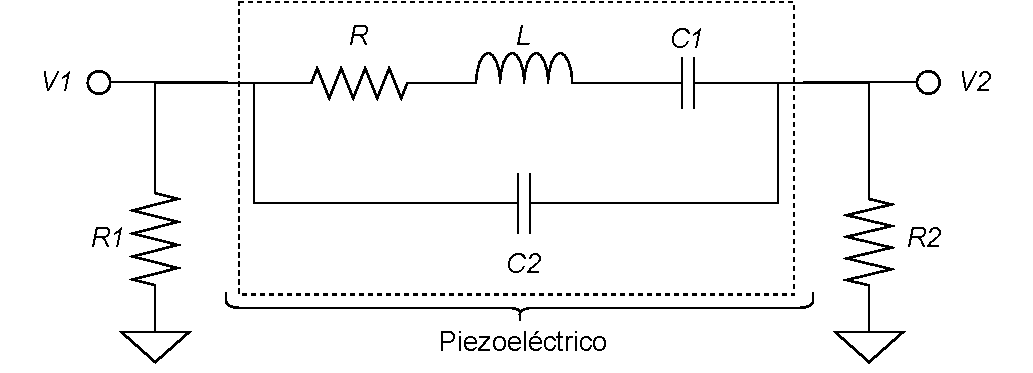
\includegraphics[width=16cm]{Circuito equivalente.drawio.pdf}
    \caption{Circuito equivalente del piezoeléctrico, considerando los
    electrodos de contacto.}
    \label{Circuito equivalente}
\end{figure}

El módulo cuadrado de la impedancia de este circuito resulta ser:

\begin{equation} \left|Z\right|^2=\frac{R^2+\left(\omega L -\frac{1}{\omega
    C_1}\right)^2}{\omega^2C_2^2R^2+\left[1-\omega C_2\left(\omega
    L-\frac{1}{\omega C_1}\right)\right]^2}= A \frac {1 + Q^2
    \bigg(\frac{\omega}{\omega_R} - \frac{\omega_R}{\omega}\bigg)^2}
{\frac{\omega^2}{\omega^2_R} + Q^2\bigg(\frac{\omega^2_A}{\omega^2_R} -
\frac{\omega^2}{\omega^2_R}\bigg)^2}\mathrm{,} \label{Impedancia piezoelectrico}
\end{equation}
donde $Q = \frac{L}{R}\omega_R$ es denominado el factor de calidad del circuito
y es una medida de la calidad del circuito como filtro pasa banda, $\omega_R =
\frac{1}{\sqrt{LC_1}}$ es la frecuencia angular de resonancia, $\omega_A =
\sqrt{\frac{1}{L}(\frac{1}{C_1} + \frac{1}{C_2})}$ la frecuencia angular de
antirresonancia, mientras que $A = \frac{1}{C^2_2\omega^2_R}$ es un parámetro
definido de manera arbitraria.
Si ademas se tienen en cuenta las resistencias $R1$ y $R2$ (Necesarias para
no dañar el piezoeléctrico), y se busca la resistencia equivalente entre $V1$ 
la tierra se tiene que esta esta dada por la ecuación \ref{Impedancia
equivalente}.
\begin{equation} \label{Impedancia equivalente}
    \left|Z_{eq}\right| = \left[\frac{1}{R_1} + \left[R_2 + \sqrt{A \frac {1 +
    Q^2 \bigg(\frac{\omega}{\omega_R} - \frac{\omega_R}{\omega}\bigg)^2}
    {\frac{\omega^2}{\omega^2_R} + Q^2\bigg(\frac{\omega^2_A}{\omega^2_R} -
    \frac{\omega^2}{\omega^2_R}\bigg)^2}}\right]^{-1}\right]^{-1}\mathrm{,}
\end{equation}                

Entonces si se midiese la caida de tension sobre $R2$ se tendri


% La transferencia de un circuito se define como la razón entre el voltaje de
% entrada y el de salida. En el caso particular del circuito de la figura
% \ref{Circuito equivalente}, esta es:

% \begin{equation}
%     T(\omega)=\frac{R_2}{\left|Z(\omega)\right|}.
% \end{equation}
% Esta expresión tiene un máximo en la frecuencia de resonancia, y un mínimo en la de antirresonancia. Básicamente, si el circuito está en resonancia, la transferencia es máxima y la impedancia es mínima. Por el contrario, si el circuito está en antirresonancia, la transferencia es mínima y la impedancia es máxima.

\section{Procedimiento experimental}
El piezoeléctrico estudiado es un monocristal de cuarzo cortado a $+5$º de uno
de los ejes cristalinos en forma de prisma de base cuadrada de $4$\,mm de lado
y \SI{50}{\milli m} de longitud, con dos de sus caras laterales metalizadas. Se
conectaron las placas metálicas a ambos extremos del piezoeléctrico a un
circuito electrónico tal como indica la figura \ref{Circuito piezoeléctrico}.
Como instrumento de medición se utilizó primero un osciloscopio y luego se
repitió el experimento con un lock-in en su lugar. Se utilizó un voltímetro
Amprobe 38XRX-A para medir las resistencias $R_1$ y $R_2$, obteniendo un valor
de  \SI{9.80(0.20)}{\kilo \ohm} para ambas. La amplitud de la tensión del
generador de funciones fue de \SI{1.000(0.011)}{V}.

\begin{figure}[H]
    \centering
    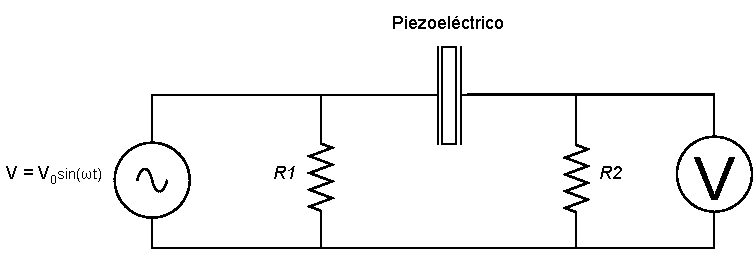
\includegraphics[width=16.5cm]{Circuito piezoeléctrico.drawio.pdf}
    \caption{Circuito utilizado para esta experiencia.}
    \label{Circuito piezoeléctrico}
\end{figure}


El procedimiento experimental consistio en variar la frecuencia de emision del
generador de funciones de manera discreta entre los \SI{49000}{Hz} y
\SI{51600}{Hz} y realizar una medicion para cada frecuencia. 

\section{Resultados}

Tras realizar las mediciones se realizo un ajuste por medio de la ecuación
\ref{Impedancia equivalente} tal como se puede apreciar en la figura
\ref{fig:voltaje y fase lock in}

\begin{figure}[H]
    \centering
    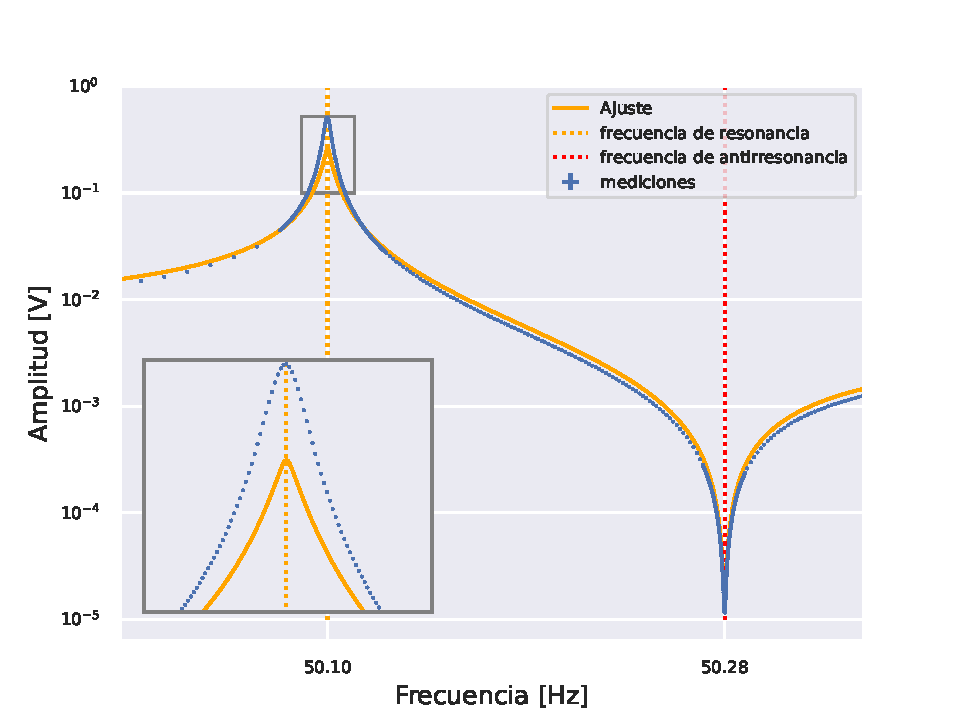
\includegraphics[width=0.8\linewidth]{amp.pdf}
    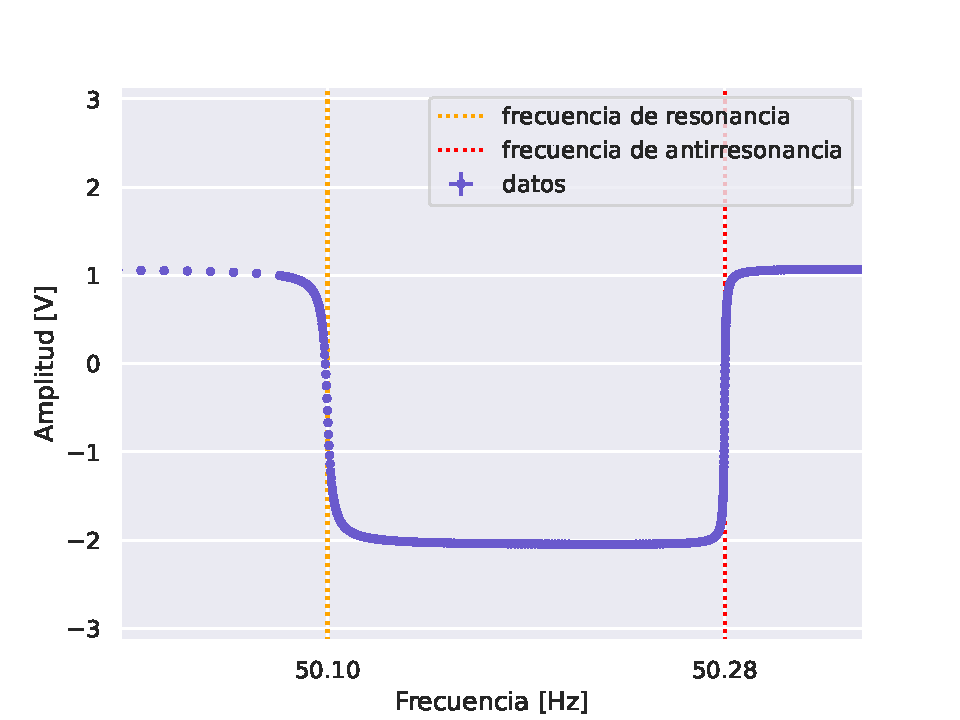
\includegraphics[width=0.8\linewidth]{phas.pdf}
    \caption{Voltaje y fase en función de la frecuencia, notese el cambio de
    $\pi$ radianes en la fase tanto en la resonancia como la antirresonancia.}
    \label{fig:voltaje y fase lock in}
\end{figure}

La frecuencia de resonancia del sistema resulto ser de
$\omega_R=$\,\SI{50092(1)}{\hertz}, mientras que la frecuencia de antirresonancia $\omega_A=$\,\SI{50280(1)}{\hertz}, el factor de calidad del Circuito
resulto ser de \SI{1}{\ohm \per \henry \per \second}

Como también se puede observar en la figura \ref{fig:voltaje y fase lock in},
el desfasaje entre las dos señales es identicamente cero cuando la frecuencia
de la onda es igual a $\omega_R$ u $\omega_A$. Esto concuerda con lo esperado,
ya que las frecuencias de resonancia o antirresonancia de un circuito se
definen como aquellas para las cuales la fase se anula

En la figura \ref{Impedancia gráfico} se puede ver graficado el módulo de la
impedancia equivalente del circuito en función de la frecuencia de la onda
emitida. Se observa fácilmente que $\left|Z\right|$ es máximo en
$\omega=\omega_A$, y mínimo en $\omega=\omega_R$, lo cual se condice con lo
esperado según la ecuación \ref{Impedancia piezoelectrico}.

\newpage

\section{Conclusiones}

Concluyendo, la respuesta de un piezoelectrico a un campo electrico variable
puede ser modelada setisfactoriamente como un circuito RLC haciendo uso de un
modelo de parametros concentrados. Para el elemento analizado en este trabajo
se observo una frecuencia de resonancia de , una frecuencia de antirresonancia
de y un factor de calidad de.

Ademas cabe a destacar que para esta clase de experiencias un amplificador
lock-in resulto ser una herramienta mucho mas conveniente que un osciloscopio,
esto se debe a los bajos voltajes involucrados los cuales suelen ser mucho
menores que las señales de ruido que se producen debido a tanto la red
electrica como campos electricos y magneticos que se puedan encontrar en el
labratorio y que el osciloscopio por si mismo no cuenta con un metodo efectivo
de aislar.

\printbibliography

\end{document}
